\maketitle
\chapter{Il Carry Save Adder Tree}
\section{Implementazione}
Dopo aver moltiplicato i pixel uscenti dalla finestra di registri per i corrispondenti valori del filtro si otterranno dunque nove operandi da 12-bit ciascuno. 

Per ottenere il pixel filtrato sarà ora necessario sommare tutti e nove gli operandi per poi avere in uscita il risultato atteso. 

Per poter fare ciò si hanno diverse strade, tra cui un classico sommatore “carta e penna” o una somma a due a due. Questi metodi, per quanto semplici da implementare, hanno però il grosso svantaggio di essere molto lenti ad effettuare il calcolo. Esistono invece metodi più efficienti che sfruttano più risorse HW ma che portano a termine l’operazione in un tempo molto più breve. Uno tra questi è l’approccio detto “Carry Save”. Questa metodologia consiste nel sommare gli operandi a due a due o a tre a tre, creando in uscita due diversi vettori contenenti rispettivamente i bit delle somme e i bit dei riporti. 

Questo approccio interrompe dunque la catena di trasporto del riporto per ogni somma, andando ad iterare questa proceduta fino ad ottenere in uscita due soli vettori da sommare. Sarà solo a questo punto che si avrà una sola catena di riporto, andando dunque a risparmiare tanto tempo a livello complessivo. Essendo questo progetto incentrato sull’efficienza, dando il giusto peso all’utilizzo delle risorse, è stato dunque scelto un approccio Carry Save per l’albero di somma mentre, per lo step finale, è stato scelto una somma mediante un modulo Carry Select Adder. Questo per via del numero di bit favorevole che ha permesso di adottare il seguente approccio senza avere sbilanciamenti o verso le troppe risorse o verso un tempo di elaborazione eccessivamente alto.

L’albero di somma sarà formato da nove operandi in ingresso corrispondenti ai prodotti parziali e saranno rappresentati da altrettanti segnali in std\_logic\_vector a 12-bit.
In uscita, per come verrà spiegato in seguito, si avrà un segnale in std\_logic\_vector a 17-bit.

\begin{figure}[H]
	\centering
	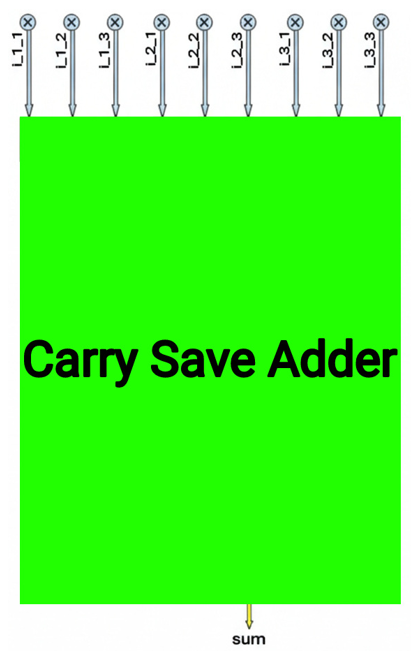
\includegraphics[width=0.5\textwidth]{file_relazione/imgs/component_csa.png}
\end{figure}

Mentre, in VHDL, il blocco sarà descritto nel seguente modo:
\begin{lstlisting}[language=VHDL, caption={Entity del circuito sommatore}]
	entity carry_save_adder_tree is
    generic (N : POSITIVE := 12);

    port (
        i_1_1, i_1_2, i_1_3 : in  std_logic_vector(
								N-1 downto 0);
        i_2_1, i_2_2, i_2_3 : in  std_logic_vector(
								N-1 downto 0);
        i_3_1, i_3_2, i_3_3 : in  std_logic_vector(
								N-1 downto 0);
        sum                 : out std_logic_vector(
								N+4 downto 0)
    );
	end carry_save_adder_tree;
\end{lstlisting}

Analizzando invece il comportamento interno del sommatore, in un primo livello i segnali verranno raggruppati a tre a tre e sommati bit a bit da un ulteriore blocco composto da dodici Full Adder separati. 

I bit in posizione i-esima daranno in uscita un bit di somma e uno di riporto che andranno nei due rispettivi vettori descritti in precedenza, senza avere dunque una catena di riporto. Dopo aver ottenuto i 12-bit di somma e riporto, il vettore dei riporti verrà shiftato a sinistra di una posizione estendendo con lo zero a destra (il LSB) e per avere lo stesso numero di bit il vettore somma verrà esteso con segno a sinistra del MSB. Questa procedura verrà ripetuta tre volte ottenendo complessivamente tre vettori di somme e tre vettori di riporti ognuno dei quali sarà a 13-bit. Graficamente la condizione può essere così descritta:
\begin{figure}[H]
	\centering
	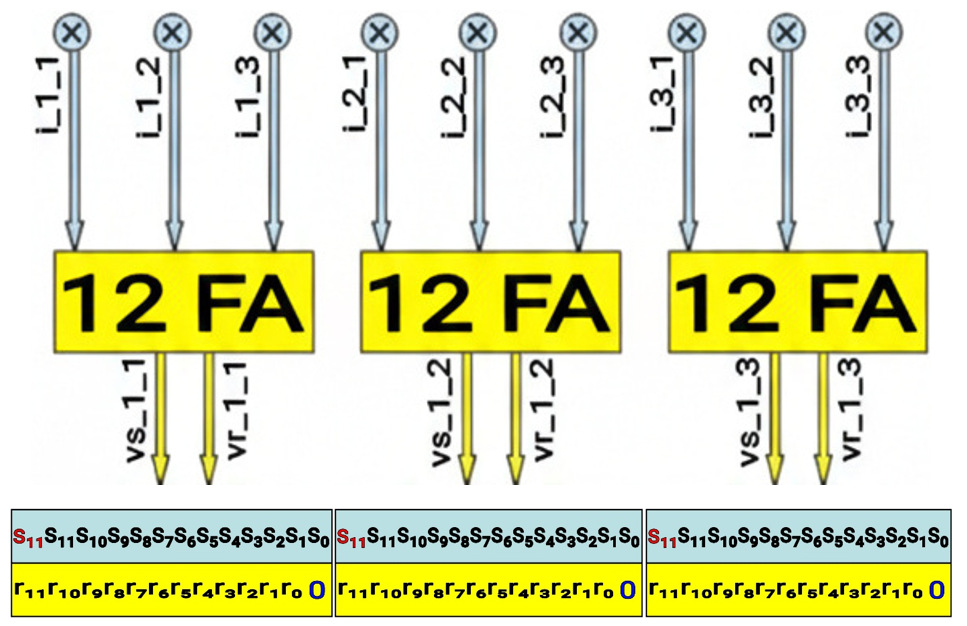
\includegraphics[width=0.9\textwidth]{file_relazione/imgs/interno_csa(1).png}
\end{figure}

È importante sottolineare che, l’estensione con lo zero a destra e l’estensione con segno a sinistra non richiede risorse aggiuntile ma solo un collegamento rispettivamente verso GND e verso il MSB.

Ottenuti i sei nuovi vettori, verrà replicata la procedura andando a raggruppare i segnali a tre a tre. Nello specifico, per il primo raggruppamento verranno presi i due segnali uscenti dal primo blocchetto e il primo del secondo blocchetto. L’altro raggruppamento sarà invece formato dal secondo segnale uscente dal secondo blocchetto e da entrambi i segnali uscenti dal terzo blocchetto.

Presi i due raggruppamenti di segnali, essi andranno in ingresso ai due nuovi blocchi sommatori. In questo secondo livello i Full Adder non saranno più dodici come prima ma tredici per via dello shift e della conseguente estensione con segno. A somme effettuate, in uscita si avranno quattro nuovi segnali, due riferiti ai vettori somma e due ai vettori riporto. Tre dei quattro segnali saranno a 14-bit e saranno i segnali di ingresso del successivo livello di somma. Il quarto segnale, quello relativo al vettore dei riporti del secondo blocchetto, avrà una doppia estensione con segno a sinistra del MSB. Esso sarà infatti l’ingresso dell’ultimo livello di somma e avrà un’estensione totale pari a 15-bit.
Graficamente la situazione sarà la seguente:
\begin{figure}[H]
	\centering
	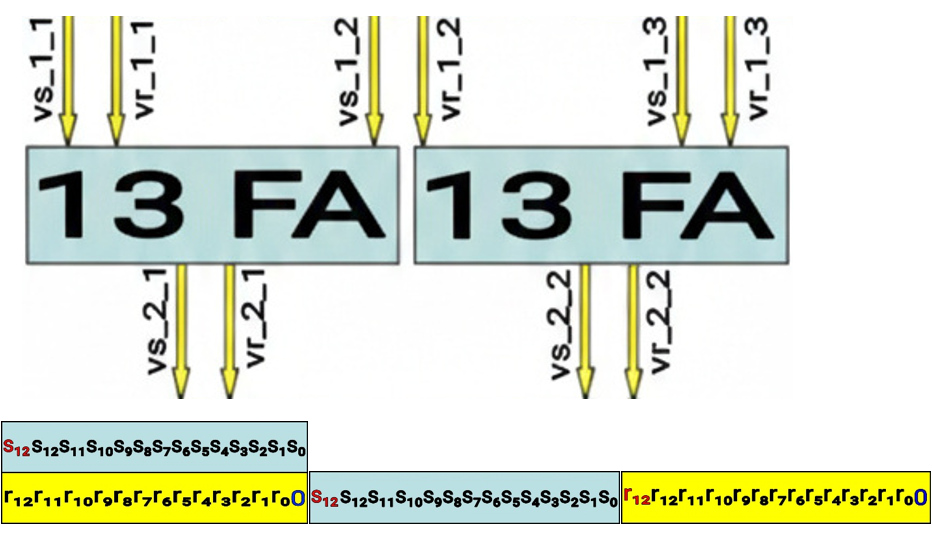
\includegraphics[width=0.9\textwidth]{file_relazione/imgs/interno_csa(2).png}
\end{figure}

Passando al successivo livello di somma, verranno presi i tre vettori da 14-bit e inviati in ingresso al blocchetto di somma composto da quattordici Full Adder mentre il segnale da   15-bit proseguirà verso il livello finale. Dal blocchetto di quattordici Full Adder usciranno ulteriori due segnali a 15-bit, uno relativo ad un vettore somma e uno al vettore riporti con le canoniche estensioni con lo zero e con segno nelle opportune posizioni. 
A livello grafico:
\begin{figure}[H]
	\centering
	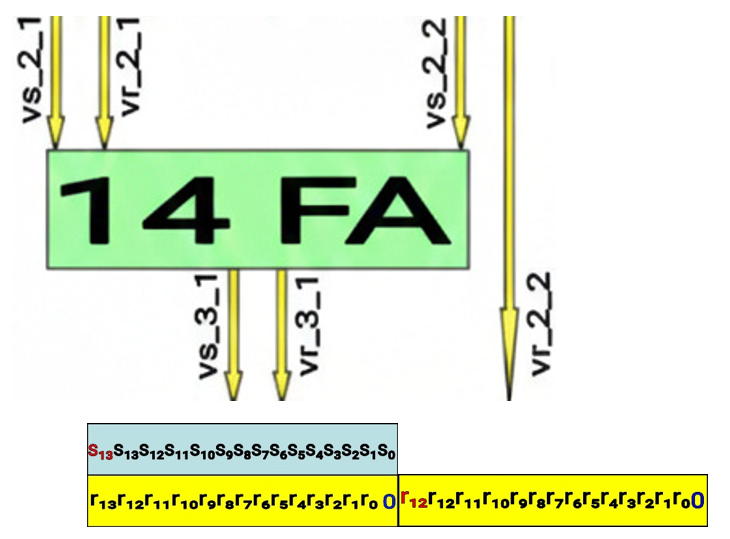
\includegraphics[width=0.9\textwidth]{file_relazione/imgs/interno_csa(3).png}
\end{figure}

A questo si arriverà ad avere tre vettori da 15-bit ciascuno, rispettivamente uno di somma e due di riporti. I tre vettori andranno in ingresso al livello di somma finale composto da quindi Full Adder che darà come uscita i due vettori finali di somma e riporto da 16-bit. 
A livello grafico:
\begin{figure}[H]
	\centering
	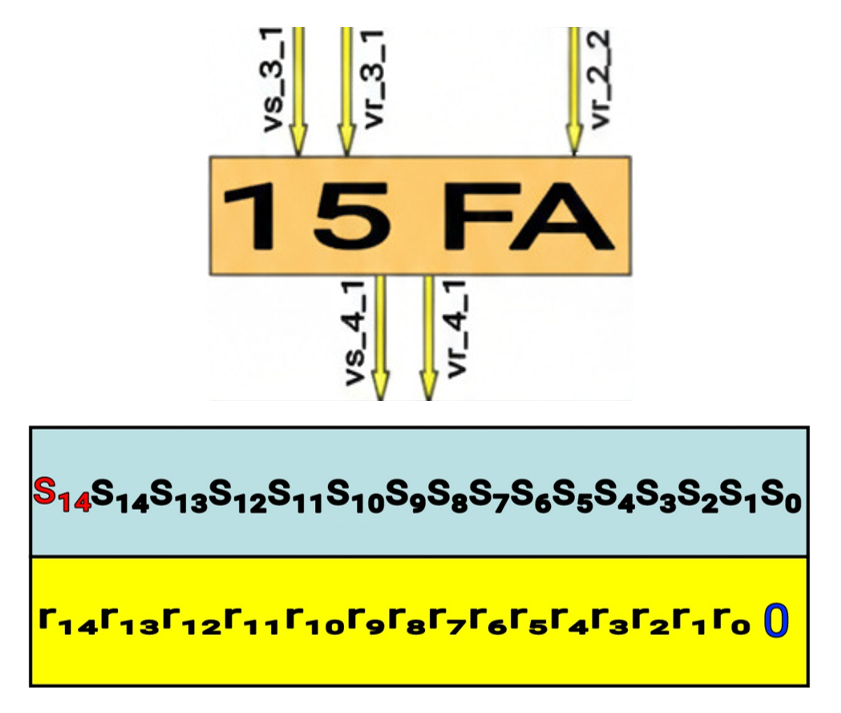
\includegraphics[width=0.9\textwidth]{file_relazione/imgs/interno_csa(4).png}
\end{figure}

Infine si avranno due vettori finali da 16-bit che, una volta sommati, daranno luogo al risultato finale. Prima di ottenere ciò andranno sommati bit a bit i due vettori con un metodo classico, e quindi con una catena di riporto.

\section{Il Carry Select Adder}
Per la seguente somma è stato scelto un Carry Select Adder con moduli di Ripple Carry Adder ad 8-bit ciascuno, trovando dunque il giusto compromesso tra risorse, potenza dissipata e tempo di elaborazione. 

Il Carry Select Adder, inoltre, sarà una versione semplificata rispetto a quella canonica poiché non faremo uso dell’ultimo riporto in uscita. Questo perché il risultato sarà a diciassette bit totali con estensione del segno a sinistra del MSB, dunque il riporto non verrà sfruttato. Essendo inoltre il riporto un segnale di selezione per il MUX del riporto, neanche quest’ultimo verrà integrato nel circuito.
\begin{figure}[H]
	\centering
	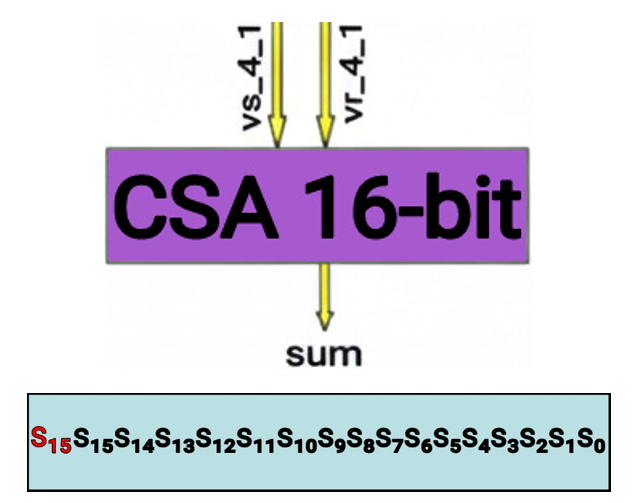
\includegraphics[width=0.9\textwidth]{file_relazione/imgs/interno_csa(5).png}
\end{figure}

 
L’implementazione del CSA in versione semplificata sarà la seguente:
\begin{figure}[H]
	\centering
	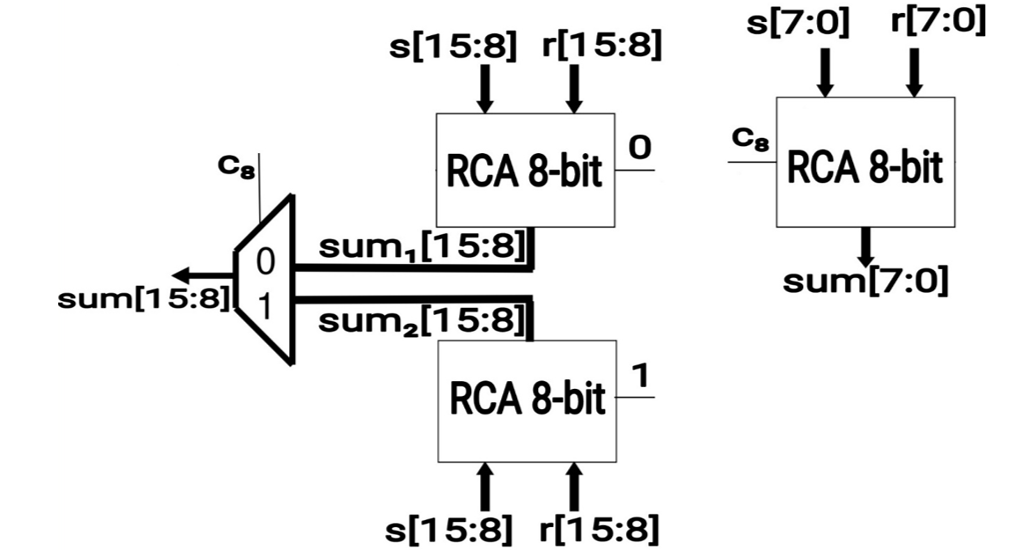
\includegraphics[width=0.9\textwidth]{file_relazione/imgs/interno_csa(6).png}
\end{figure}

\section{Il circuito finale}
Unendo tutte le varie parti si otterrà dunque il seguente circuito, corrispondente ad un sommatore a nove operandi da dodici bit ciascuno con approccio Carry Save Adder e sommatore a Carry Select Adder finale:
\begin{figure}[H]
	\centering
	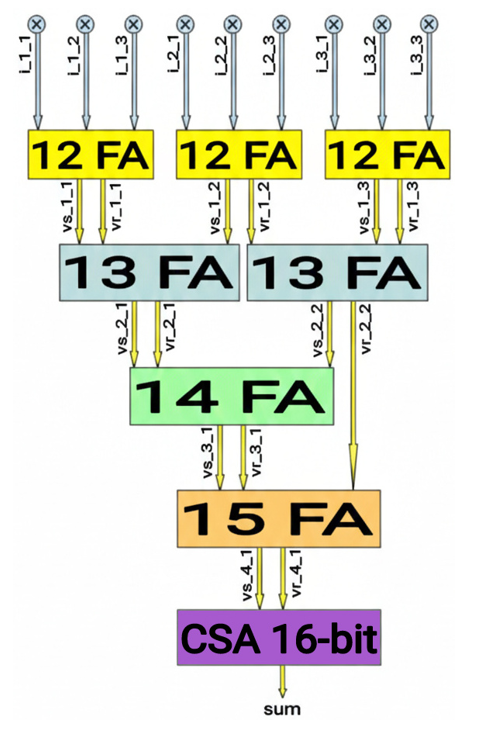
\includegraphics[width=0.75\textwidth]{file_relazione/imgs/csa.png}
\end{figure}